\chapter{Toy Monte Carlo for Systematics Studies}

Studies of systematics for experiments is generally a difficult process as multiple different effects need to be taken into account.
It is not a trivial problem to determine how uncertainty in one parameter will propagate into a systematic uncertainty on a final result.
For example, an error in the resolution affects how the fit, which is calculated over thousands of channel-dataset pairs, will resolve events near the Q-value.
The only parameter in CUORE that propagates ``easily" is the uncertainty on the efficiency, which affects the result in a simple, linear fashion. However, other parameters, such as the resolution, are, in general, intractable algebraically.
These can be studied directly, however, by performing pseudo-experiments, called Toy Monte Carlo, on generated datasets based on real data that have been perturbed by the uncertainty in a parameter.
For example, to study the effect of uncertainty on the Q-value, pseudo-experiments are performed with a generated signal centered with the Q-value perturbed by the uncertainty (here, 0.5 keV higher and lower) to see how that would have affected the measurement of the signal.


\section{Toy Monte Carlo Overview}

The idea behind pseudo-experiments is a simple one.
If there were a thousand universes each with their own CUORE and taking data for exactly the same amount of time, one would expect to see a thousand different results spread around the ``real" physical result.
However, only one of these results can be observed, so by working backwards, these other results can be replicated to study their features.
For instance, systematic biases such as the bias due to the fit can be straightforwardly studied through the use of these pseudo-experiments.
By scaling up the ``true" signal rate in pseudo-experiments, the fit bias can be directly understood and characterized.

\section{Toy Monte Carlo for Neutrinoless Double Beta Decay Search}

The generation and fitting procedure for Toy Monte Carlo can be summed up with the following steps:
\begin{enumerate}
\item Fit the real data, $D_0$.
\item Create a model, $H_0$, from the fit to real data.
\item \label{item:generate} From $H_0$, generate new data, $D_i$. Repeat to create as many Toy Monte Carlo as needed. Do not Poisson-float the number of events when determining the p-value.
\item Fit each $D_i$ with the same fitting process as was done to $D_0$.
\item See how parameters from $H_0$ compare with $H_i$
\end{enumerate}

In the case for \autoref{ssec:Fit Biases} and \autoref{ssec:Systematic Calculations}, this process is slightly different. There, the model needs to be perturbed in some manner when generating the data, so \autoref{item:generate} would then include an alteration of $H_0$ to a new model $H_1$ where the parameter has been perturbed.

Also, the choice of the model to use $H_0$ can be up for some debate. In order to keep the analysis blinded, it is important to finalize the method used beforehand. While for the first PRL paper, we decided to use the fit to data with the signal rate fixed to zero (the null hypothesis) as the base fit to use to calculate all the systematics, it would be better to use the fit to the data with a floating signal rate as the base fit to calculate systematics. Naturally, to evaluate the p-value, one should use the null hypothesis model.


\section{Toy MC Tests}
\subsection*{Goodness-of-fit Tests}
\label{sec:Goodness-of-fit}
One use of Toy MC is to determine how good a particular fit is to the data, particularly at how Poisson fluctuations of the data would affect the fit statistics.
In CUORE, we do this tests with two different methods. One of which is the Kolmogorov-Smirnov (K-S) Test statistic, given by
\begin{eqnarray}
D_n = \sup|F(x) - F_{obs}(x)| 
\end{eqnarray}
where $F_{obs}$ is the cumulative distribution function of the observed data, and $F(x)$ is the cdf of the model in consideration. In this case, it is a cdf of the fit model to the (pseudo)data. An example is shown in \autoref{fig:ksstat}.

The other statistic used to test is the negative log likelihood (NLL) for each of the fits to the ToyMC, shown in \autoref{fig:nll}. This is the (negative) sum of the log likelihoods of the data given a Poisson distribution, namely,
\begin{eqnarray}
L(\lambda; x_1,...,x_n) = -n\lambda - \sum_{j=1}^{n}\ln(x_j!) +\ln(\lambda) \\
-L(\lambda; x_1,...,x_n) = n\lambda + \sum_{j=1}^{n}\ln(x_j!) -\ln(\lambda)
\end{eqnarray}
where lambda is the expected value for the data in a particular bin, $j$, and $x_j$ is the actual data in that bin.
Maximizing the log likelihood (or minimizing the negative log likelihood) is a commonly-used method for fitting, as the log likelihood can be used as an extremum estimator. 
For CUORE, we perform an unbinned fit, which can be thought of intuitively as the limit where all the bins are infinitely small, but the underlying idea is the same.

\begin{figure}
\centering
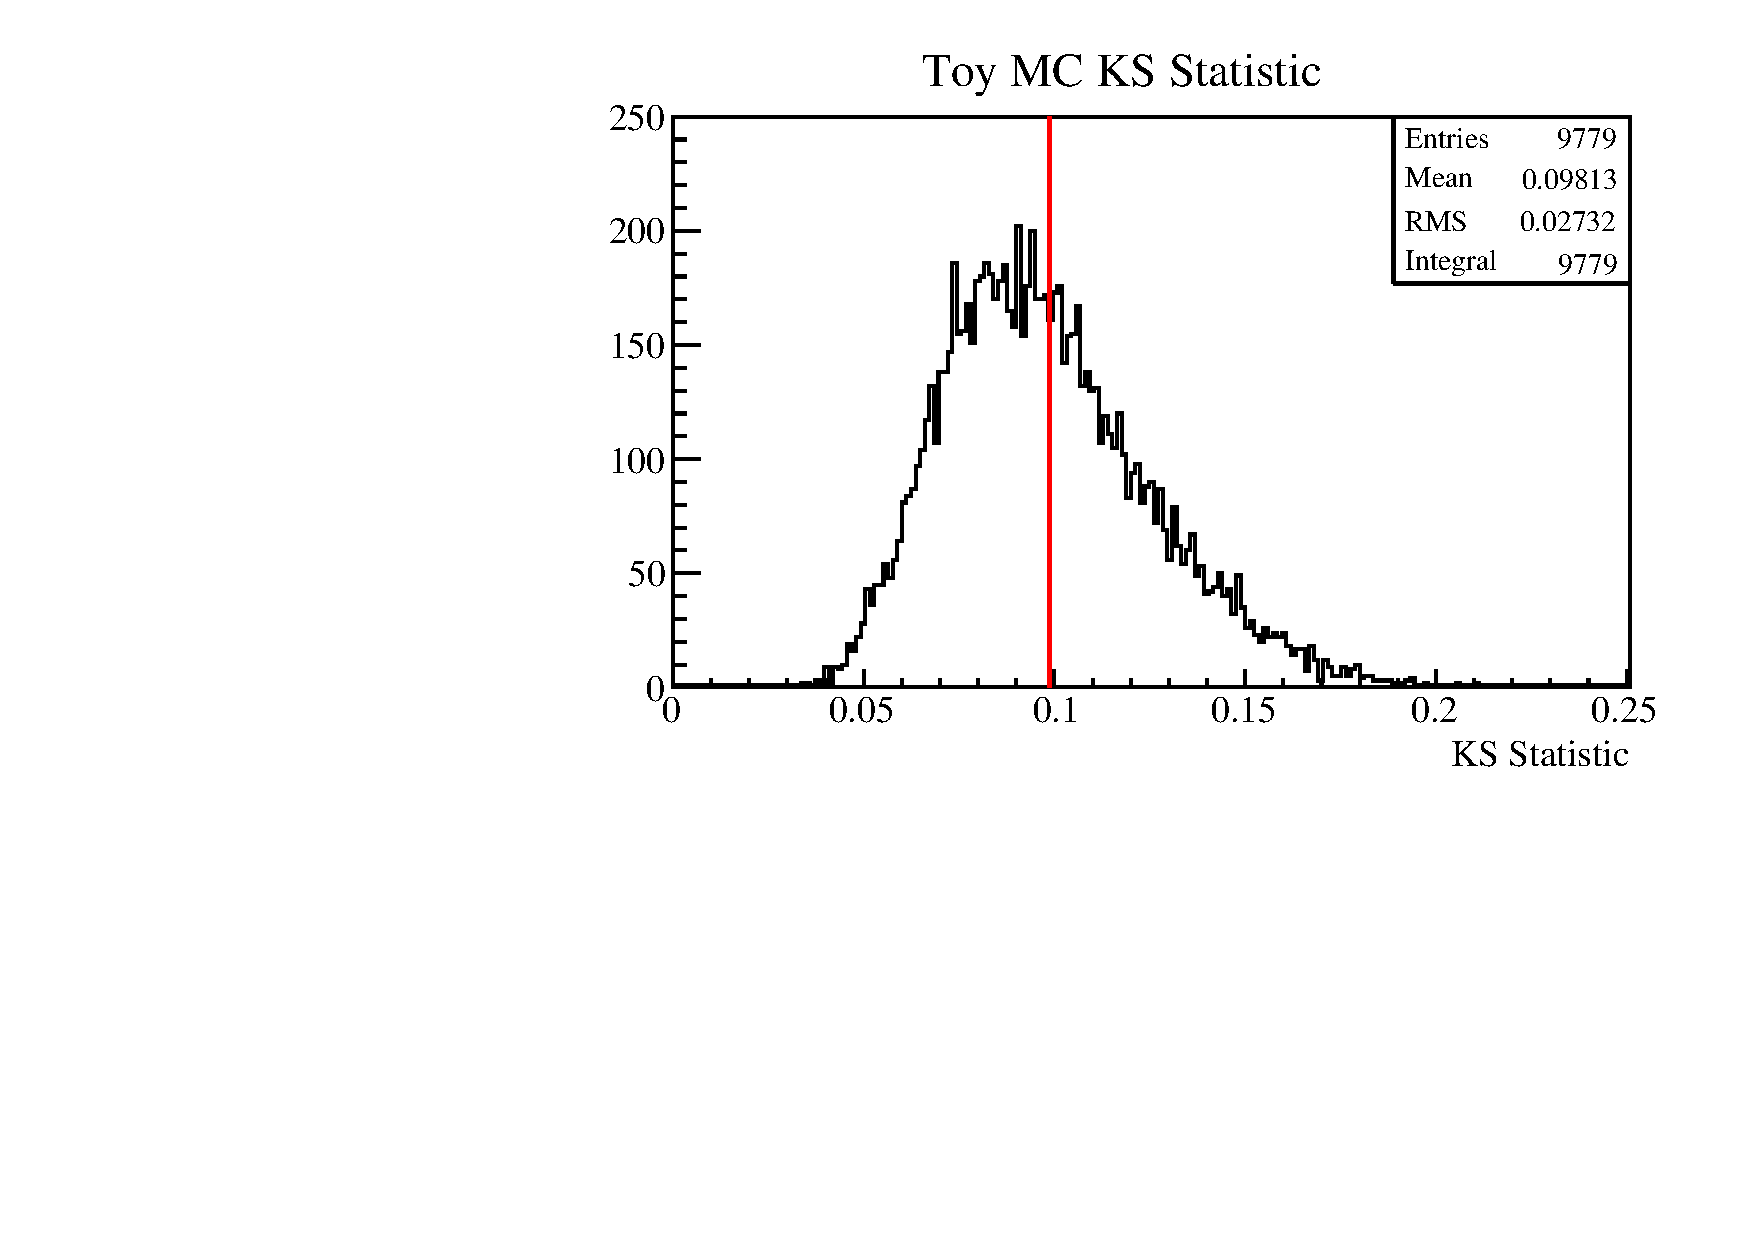
\includegraphics[width=0.7\linewidth]{Figures/Appendix_Figures/KSStat_NoPoisson.pdf}
\caption[The sample K-S distribution for 10k Toy MC]
{The sample K-S distribution for 10k Toy MC. The value from the fit to real data is marked in red.
As the fit of the real data is similar to the mean of the distribution of the K-S statistic and small, the fit is said to be good.}
\label{fig:ksstat}
\end{figure}

\begin{figure}
\centering
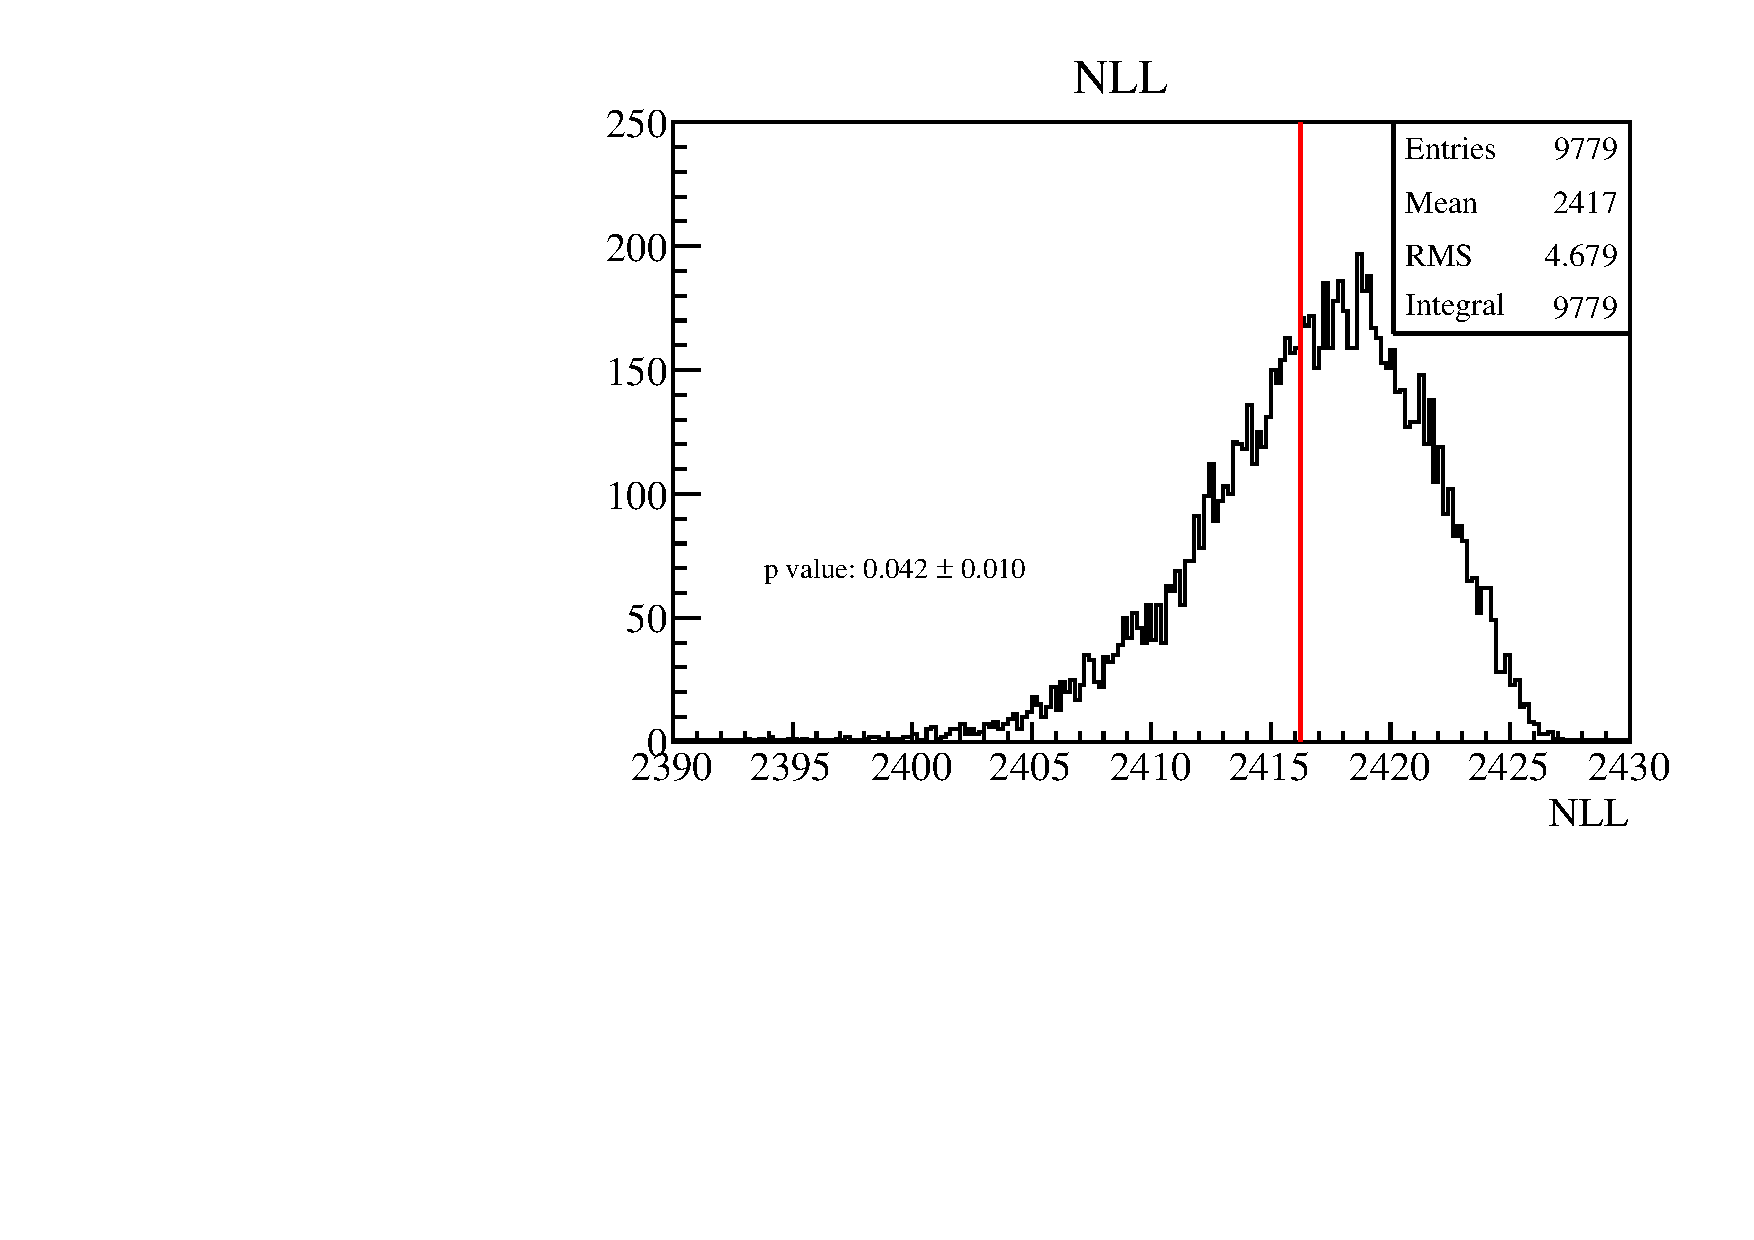
\includegraphics[width=0.7\linewidth]{Figures/Appendix_Figures/NLL_Pvalue_NoPoisson.pdf}
\caption[The NLL distribution for 10k Toy MC]
{The NLL distribution for 10k Toy MC.
The value from the fit to real data is marked in red.}
\label{fig:nll}
\end{figure}


\subsection*{Fit Biases}
\label{ssec:Fit Biases}
As mentioned previously, another use of the Toy MC is to determine bias to the fits.
In particular, in a fit to Toy MC generated without any signal ought to reconstruct, on average, zero signal with a roughly gaussian shape.
Any deviation from zero in this case can be detected by finding the mean of the distribution of signal rates from the ToyMC and by determining the distribution of the pulls of the rates, shown in \autoref{fig:signalrate} and \autoref{fig:signalpulls} respectively.
\begin{figure}
\centering
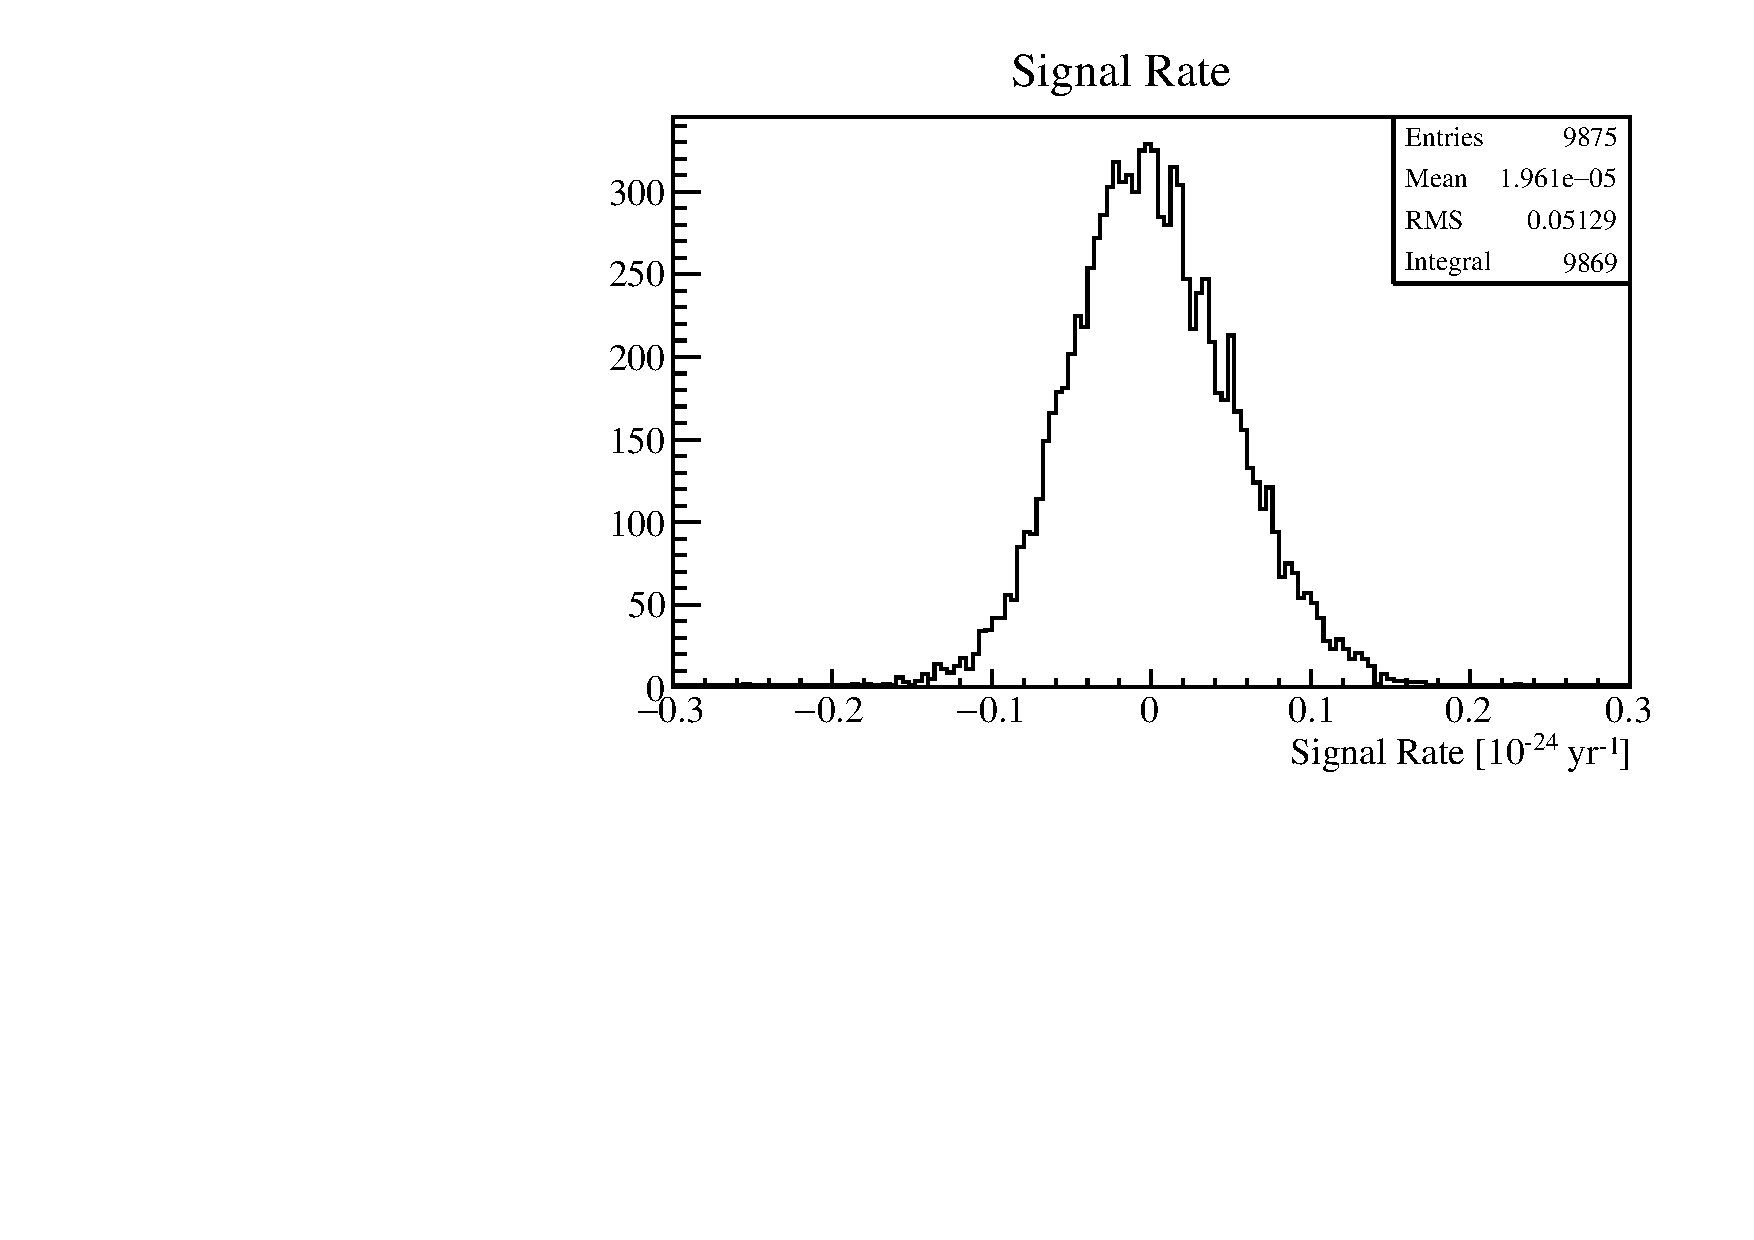
\includegraphics[width=0.7\linewidth]{Figures/Appendix_Figures/SignalRate.pdf}
\caption[The fitted signal rate for Toy Monte Carlo produced with the signal rate in $H_1$ set to zero]
{The fitted signal rate for Toy Monte Carlo produced with the signal rate in $H_1$ set to zero.
The mean of the fit is zero, as expected, but there is a longer tail towards positive signal.}
\label{fig:signalrate}
\end{figure}

\begin{figure}
\centering
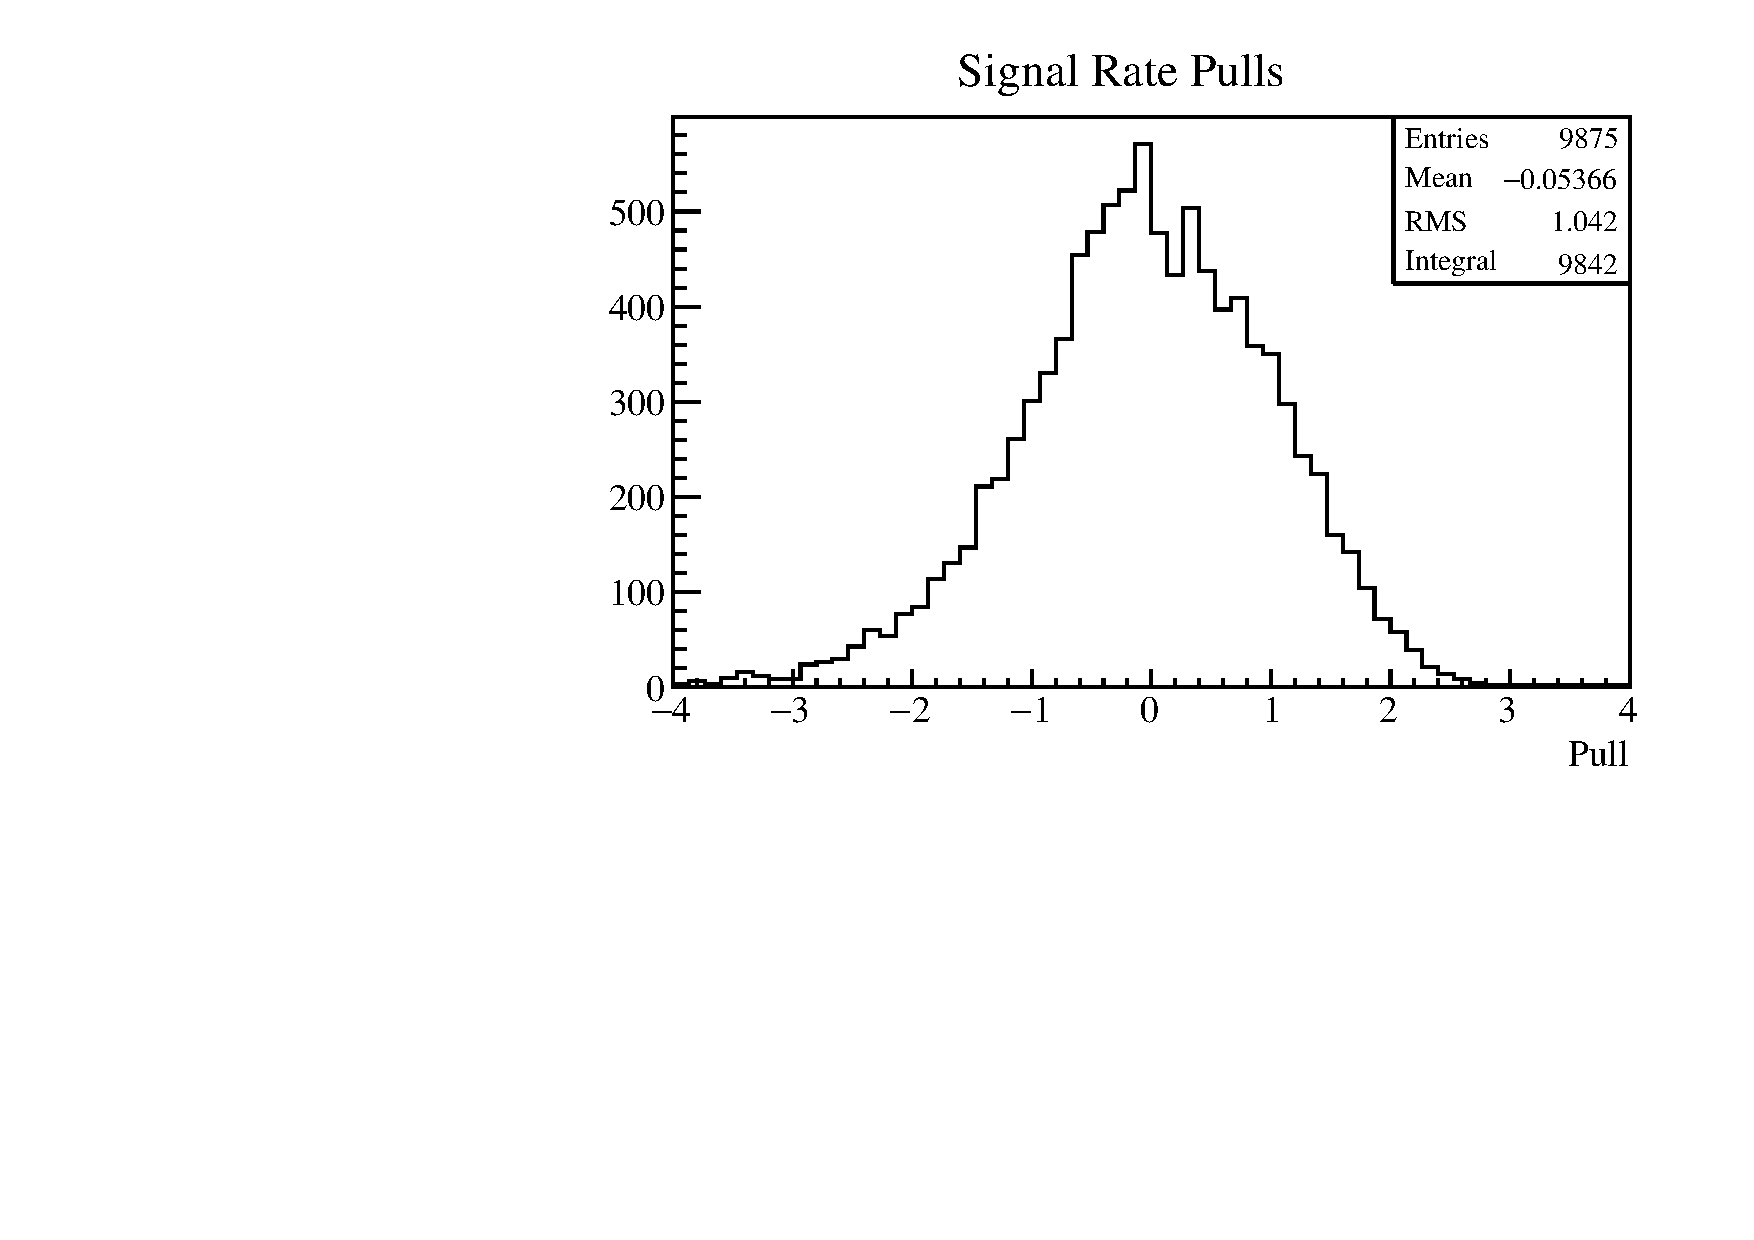
\includegraphics[width=0.7\linewidth]{Figures/Appendix_Figures/SignalPulls.pdf}
\caption[The pulls for the distribution shown in \autoref{fig:signalrate}]
{The pulls for the distribution shown in \autoref{fig:signalrate}.
While the signal rate has a tail to the right, the pulls have a tail to the left.}
\label{fig:signalpulls}
\end{figure}
In addition to the signal rates, this procedure can also be used to investigate other parameters such as the background, shown in \autoref{fig:bkgrate3021} and \autoref{fig:bkg3021pulls}.
This can be calculated for each dataset's background rates.

\begin{figure}
\centering
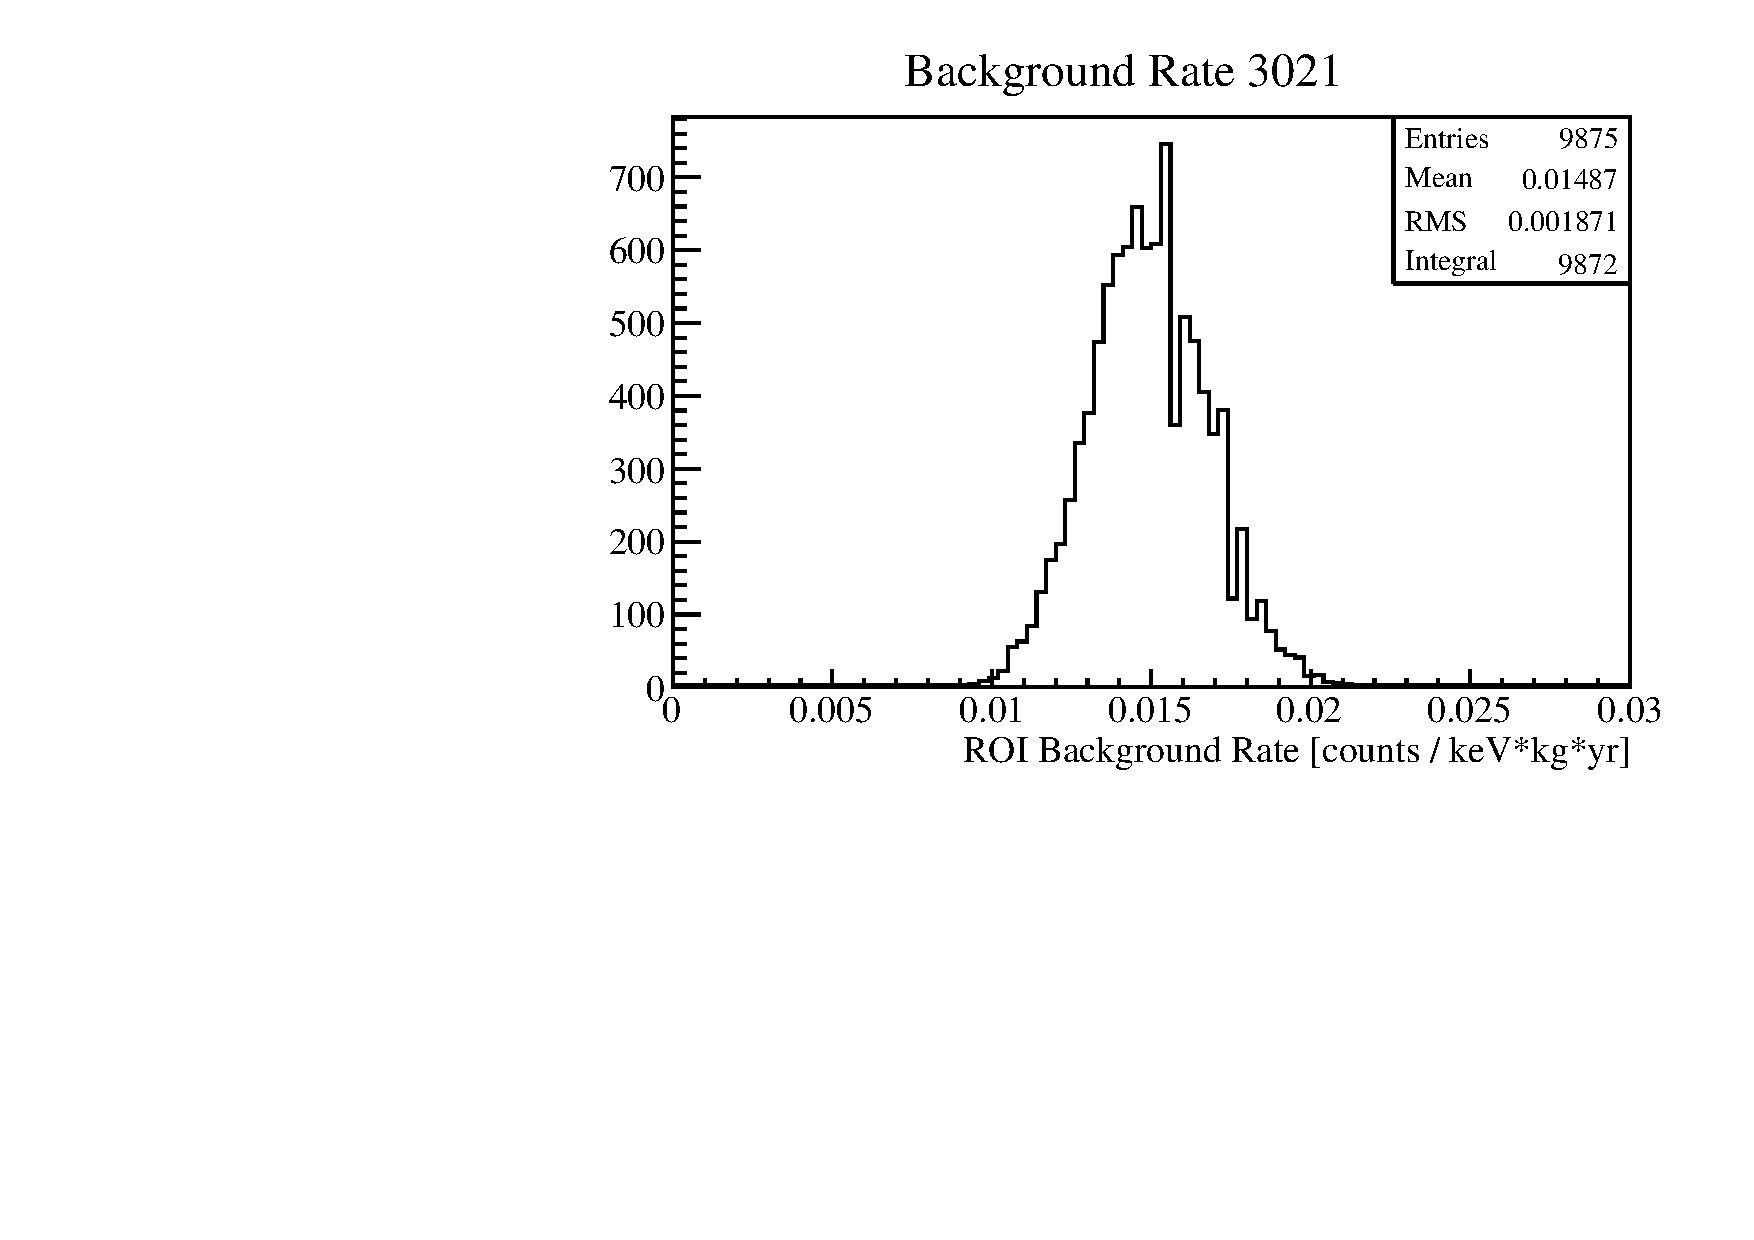
\includegraphics[width=0.7\linewidth]{Figures/Appendix_Figures/Bkg3021Rate.pdf}
\caption[The fitted background rates for Toy Monte Carlo generated with $H_1$ fixed with a signal rate of 0]{The fitted background rates for Toy Monte Carlo generated with $H_1$ fixed with a signal rate of 0.
The distribution is not expected to look Gaussian or Poisson, and the pulls of the distribution are shown in \autoref{fig:bkg3021pulls}.}
\label{fig:bkgrate3021}
\end{figure}

\begin{figure}
\centering
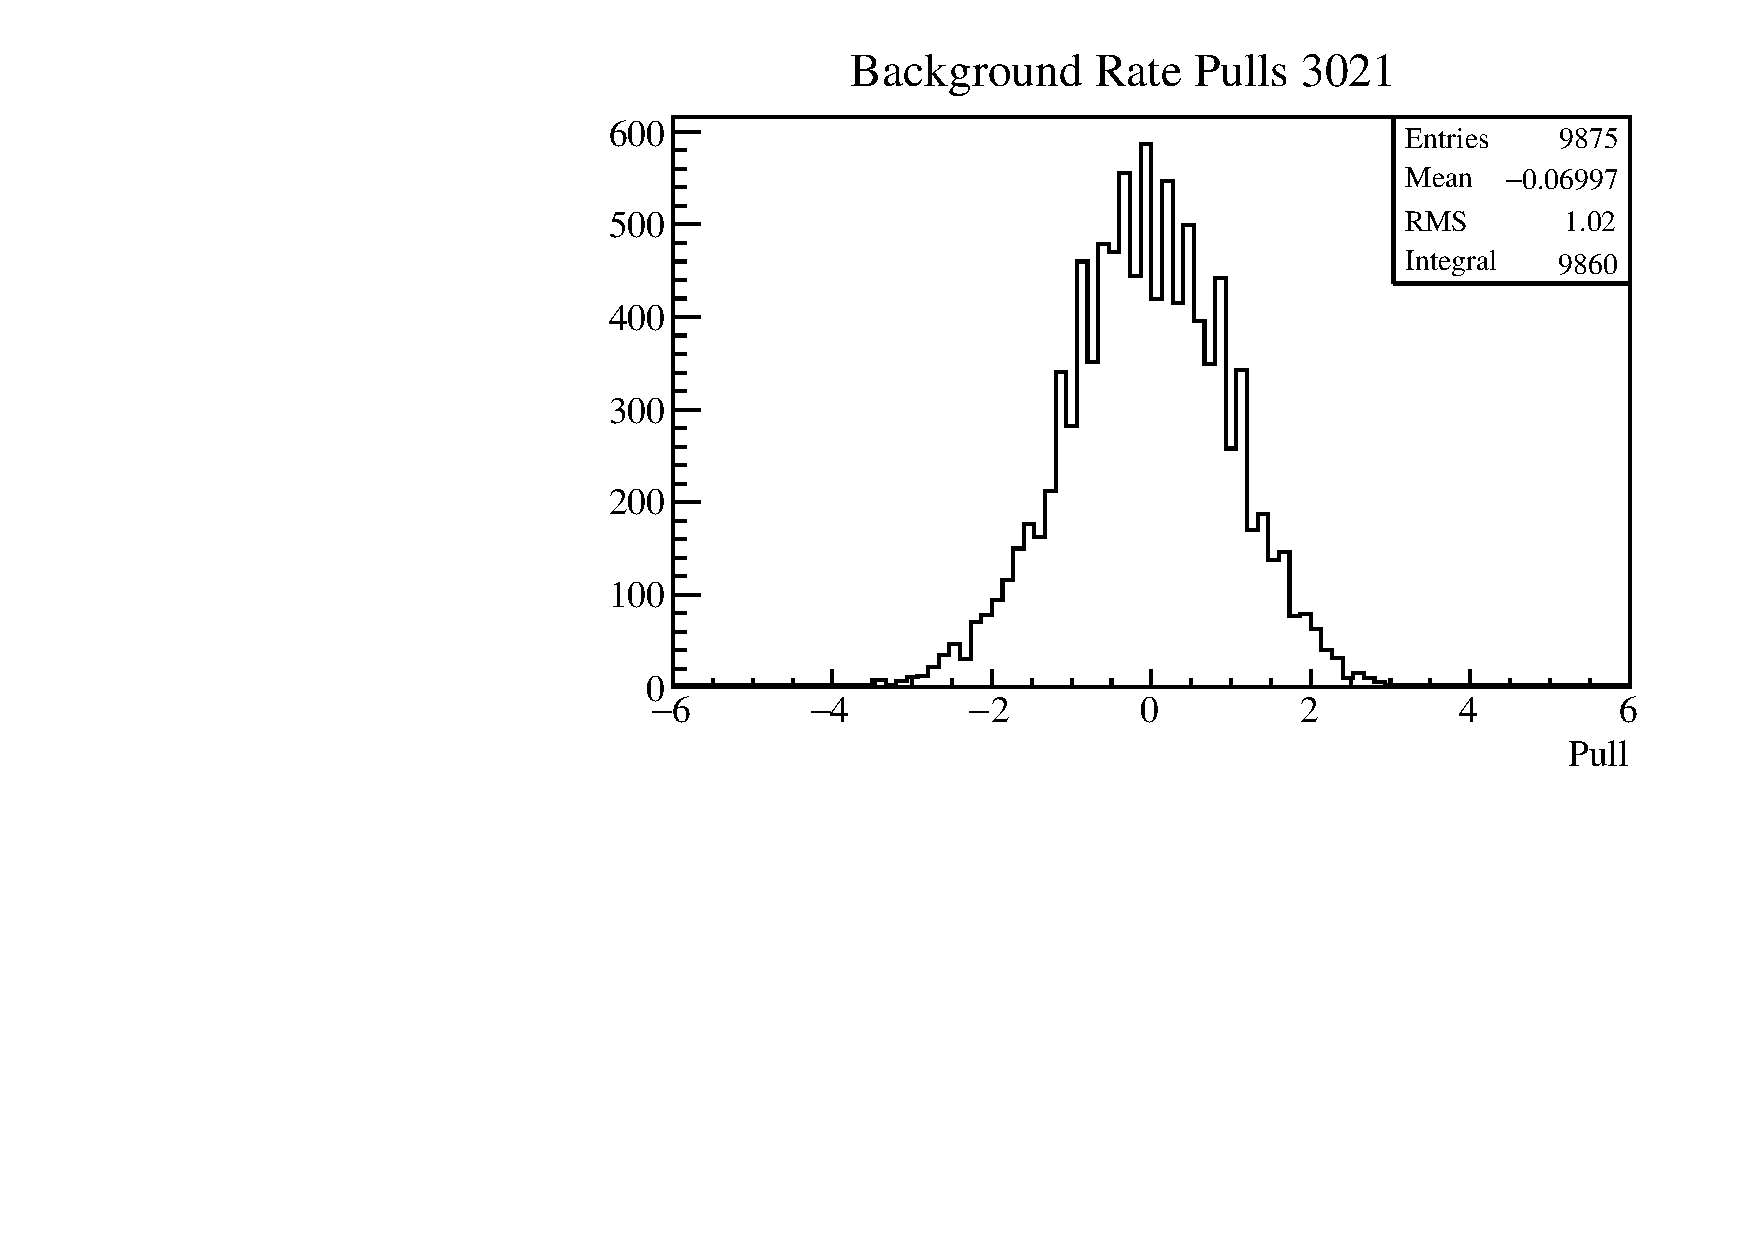
\includegraphics[width=0.7\linewidth]{Figures/Appendix_Figures/Bkg3021Pulls.pdf}
\caption{The pulls calculated for the background rate in \autoref{fig:bkgrate3021}.
The pull here is mostly Gaussian, so the fit looks okay.}
\label{fig:bkg3021pulls}
\end{figure}

\subsection*{Systematic Calculations}
\label{ssec:Systematic Calculations}
Building off the fact that the mean of the distribution of the fitted signal rates should match the generated ``true" value input in generating pseudodata, this can be used to calculate systematic errors on CUORE data for certain parameters we input in the ToyMC.
In particular, these systematic effects are studied for the fit for \zeronubb:
\begin{itemize}
\item Fit Bias
\item Linear background
\item Q-value location
\item Efficiency
\item 2615 keV lineshape parameters
\end{itemize}

To calculate the systematic effects on the measurement due to each of these parameters, pseudodata is generated via a pdf modulated by a $\pm1\sigma$ difference on each of the parameters, and signal rates are fit and plotted as a function of the ``true" signal rate input in the generated Toy MC.
A linear fit then parametrizes the systematic bias to be a flat absolute bias plus a linear relative bias term, calculated as:
\begin{equation}
y = (\textrm{relative bias}+1) \cdot x + \textrm{absolute bias}.
\end{equation}
For a parameter that has no bias on the fit, it would have a simple linear fit of 
\begin{equation}
y = 1\cdot x + 0.
\end{equation}
In particular, the existence of a relative bias means that the fitted value for signal depends on the strength of the signal, and an absolute bias is an effect that does not depend on the `true' signal.
To be conservative, the higher of the linear fit bias or its fitted error is taken for the bias in the fit.
These linear fits to determine the bias for the systematics listed above are shown in \autoref{fig:signalbias}, \autoref{fig:linearhigh}, \autoref{fig:qvaluehigh}, and \autoref{fig:nosubpeaks}.
\begin{figure}
\centering
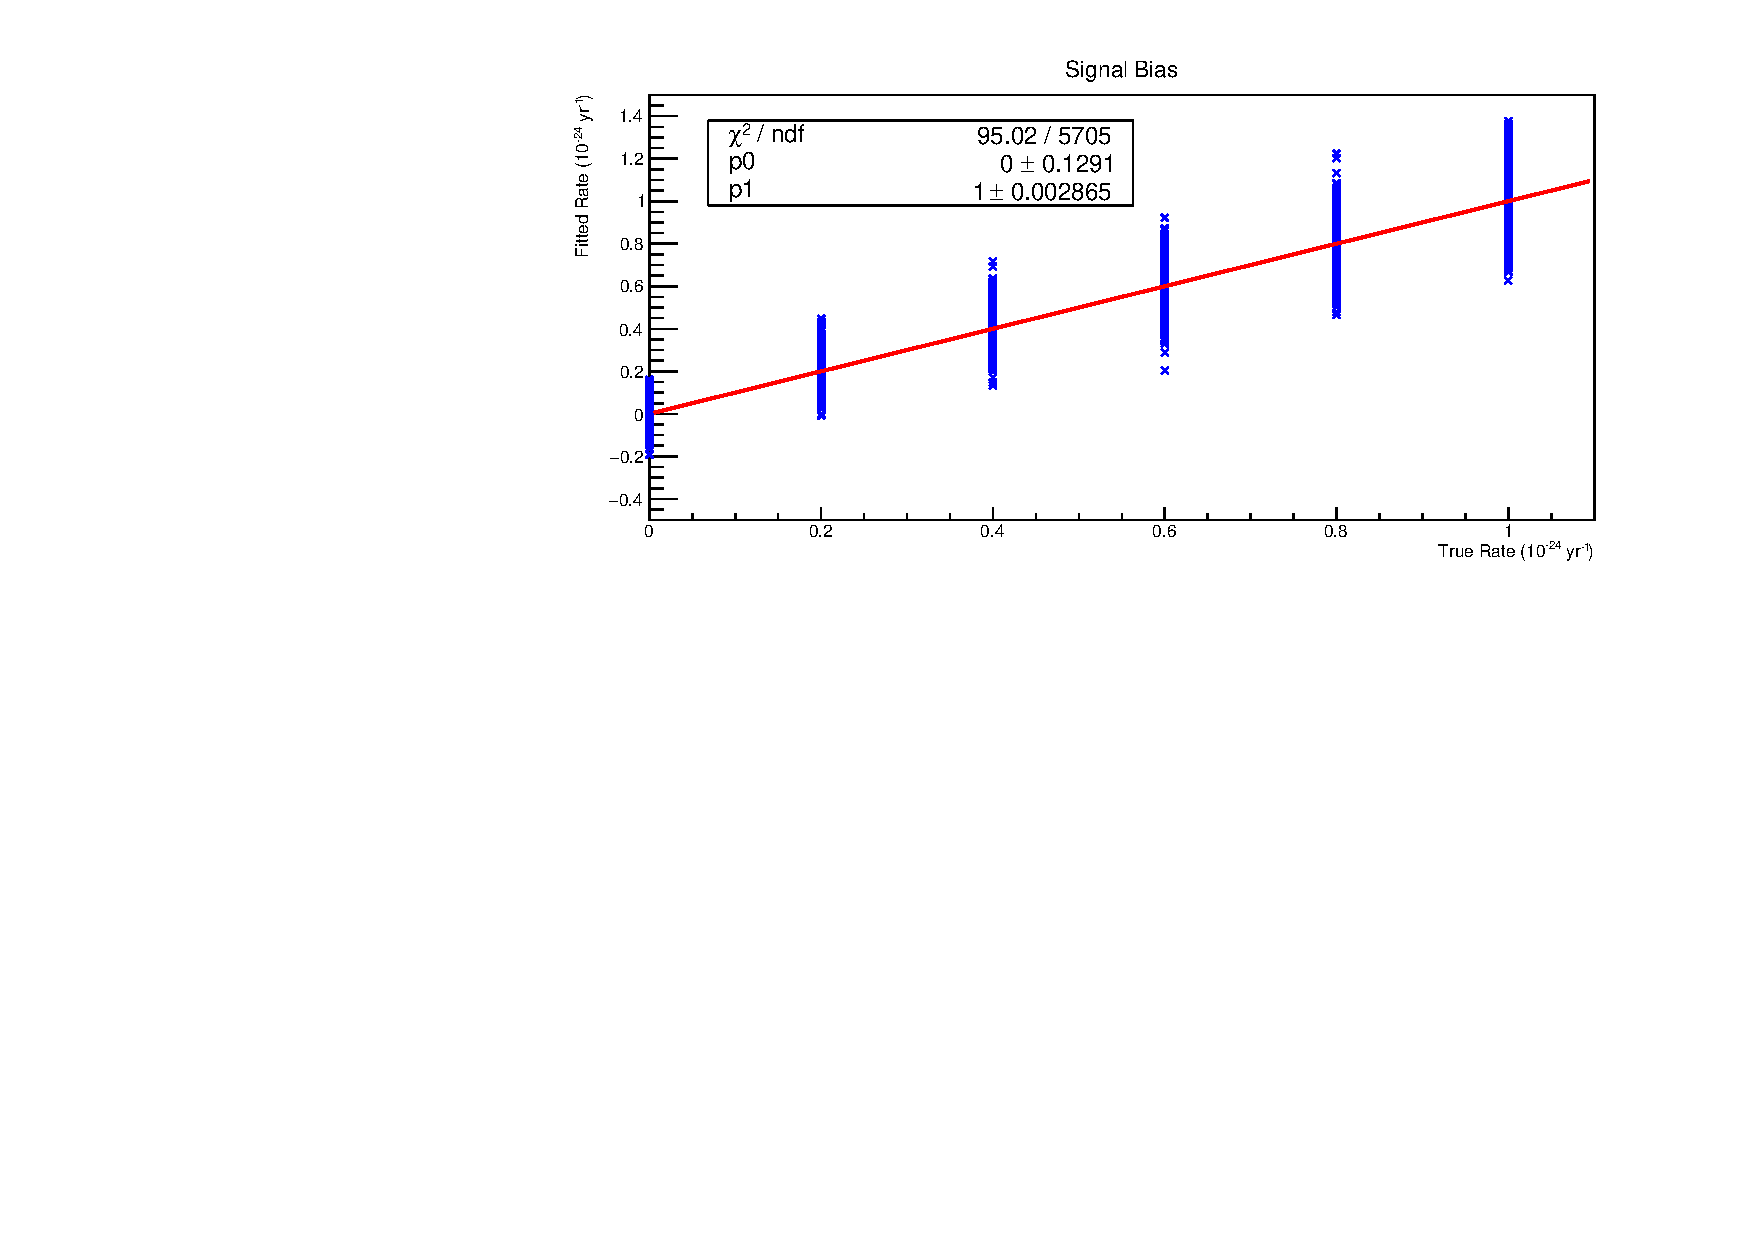
\includegraphics[width=0.7\linewidth]{Figures/Appendix_Figures/SignalBias.pdf}
\caption[The fitted signal rate as a function of the input signal rate without any other parameters adjusted]
{The fitted signal rate as a function of the input signal rate without any other parameters adjusted.
From \autoref{fig:signalrate}, the absolute bias is fixed to 0, and no relative bias is observed.
A conservative 0.3\% relative uncertainty is applied from the error on the linear fit.}
\label{fig:signalbias}
\end{figure}

\begin{figure}
\centering
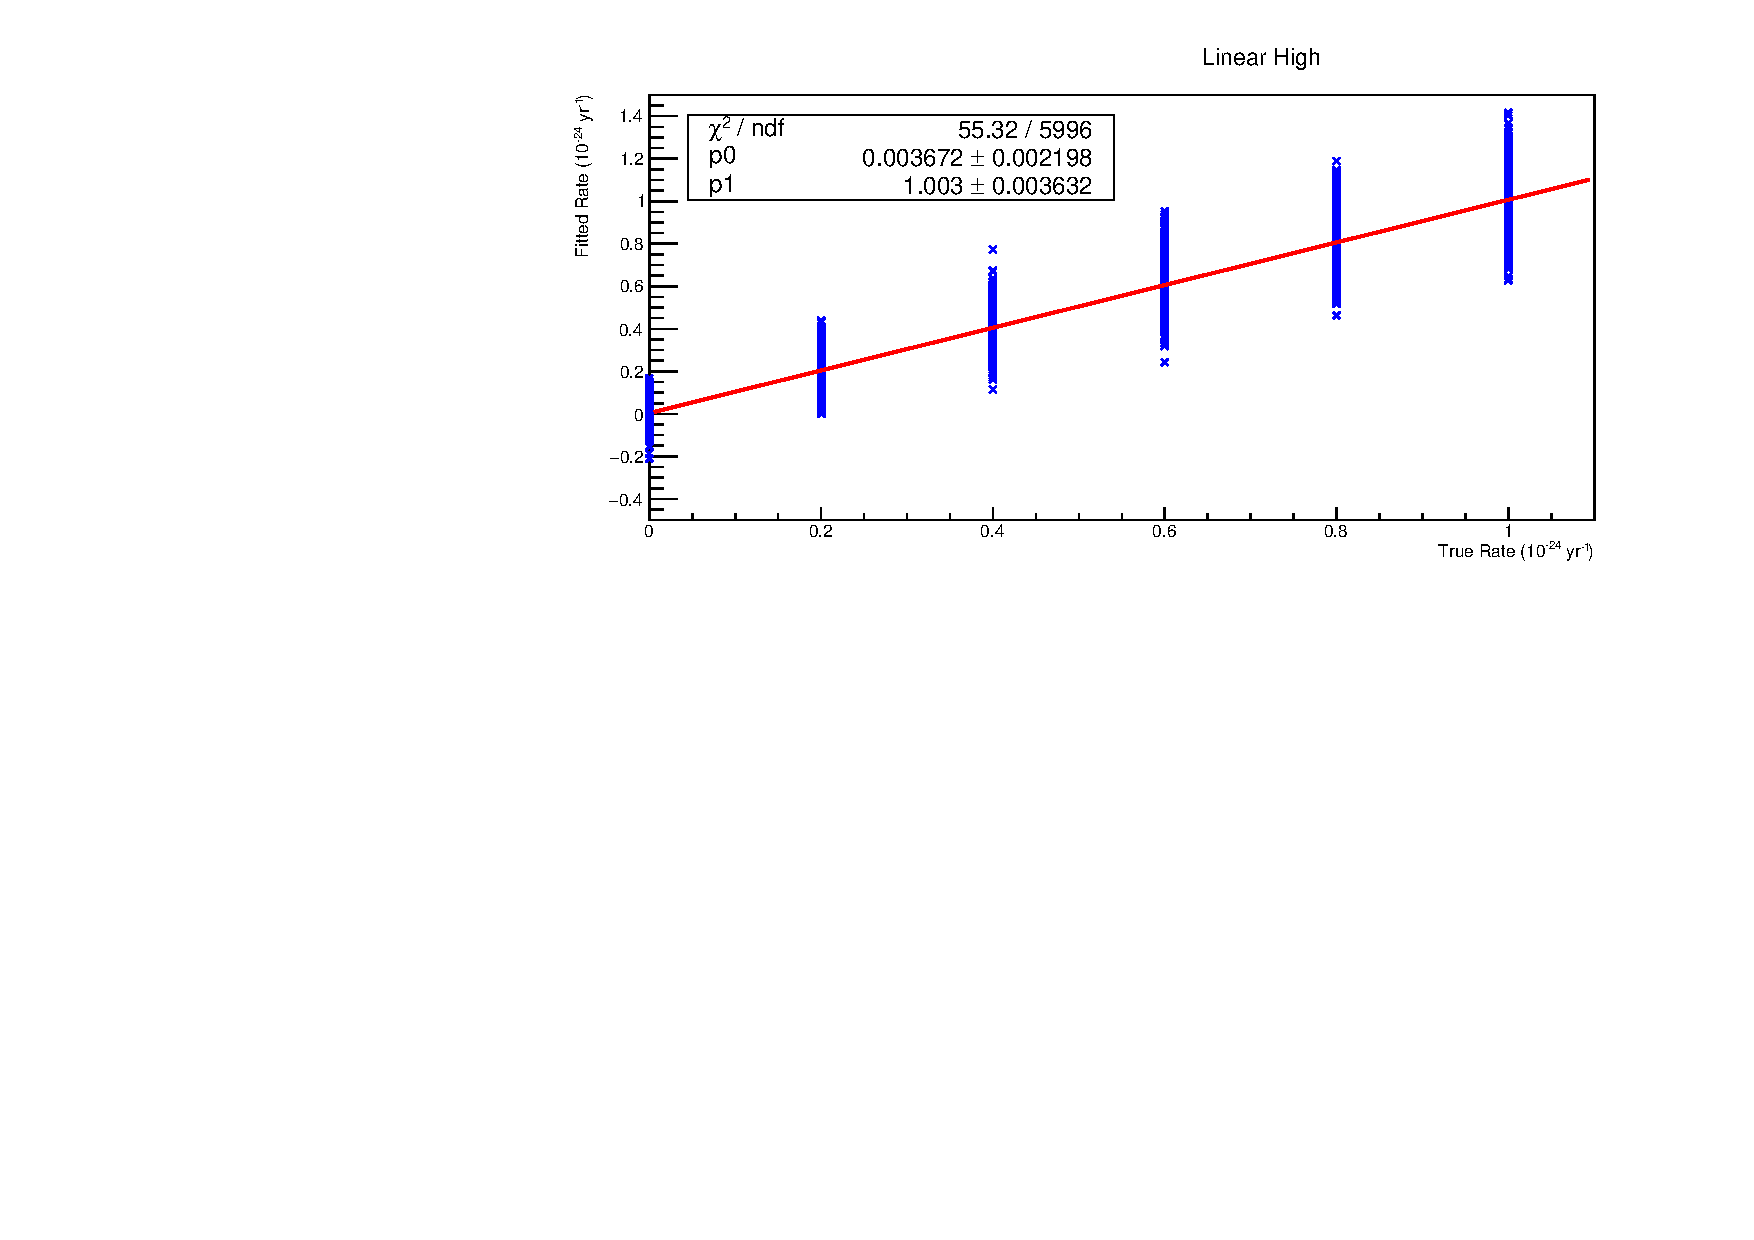
\includegraphics[width=0.7\linewidth]{Figures/Appendix_Figures/LinearHigh.pdf}
\caption[The fitted signal rate with the addition of a positive linear background nuisance parameter]
{The fitted signal rate with the addition of a positive linear background nuisance parameter.
This provides both an absolute and relative bias on the fit.
A similar plot results from a negative linear background.}
\label{fig:linearhigh}
\end{figure}

\begin{figure}
\centering
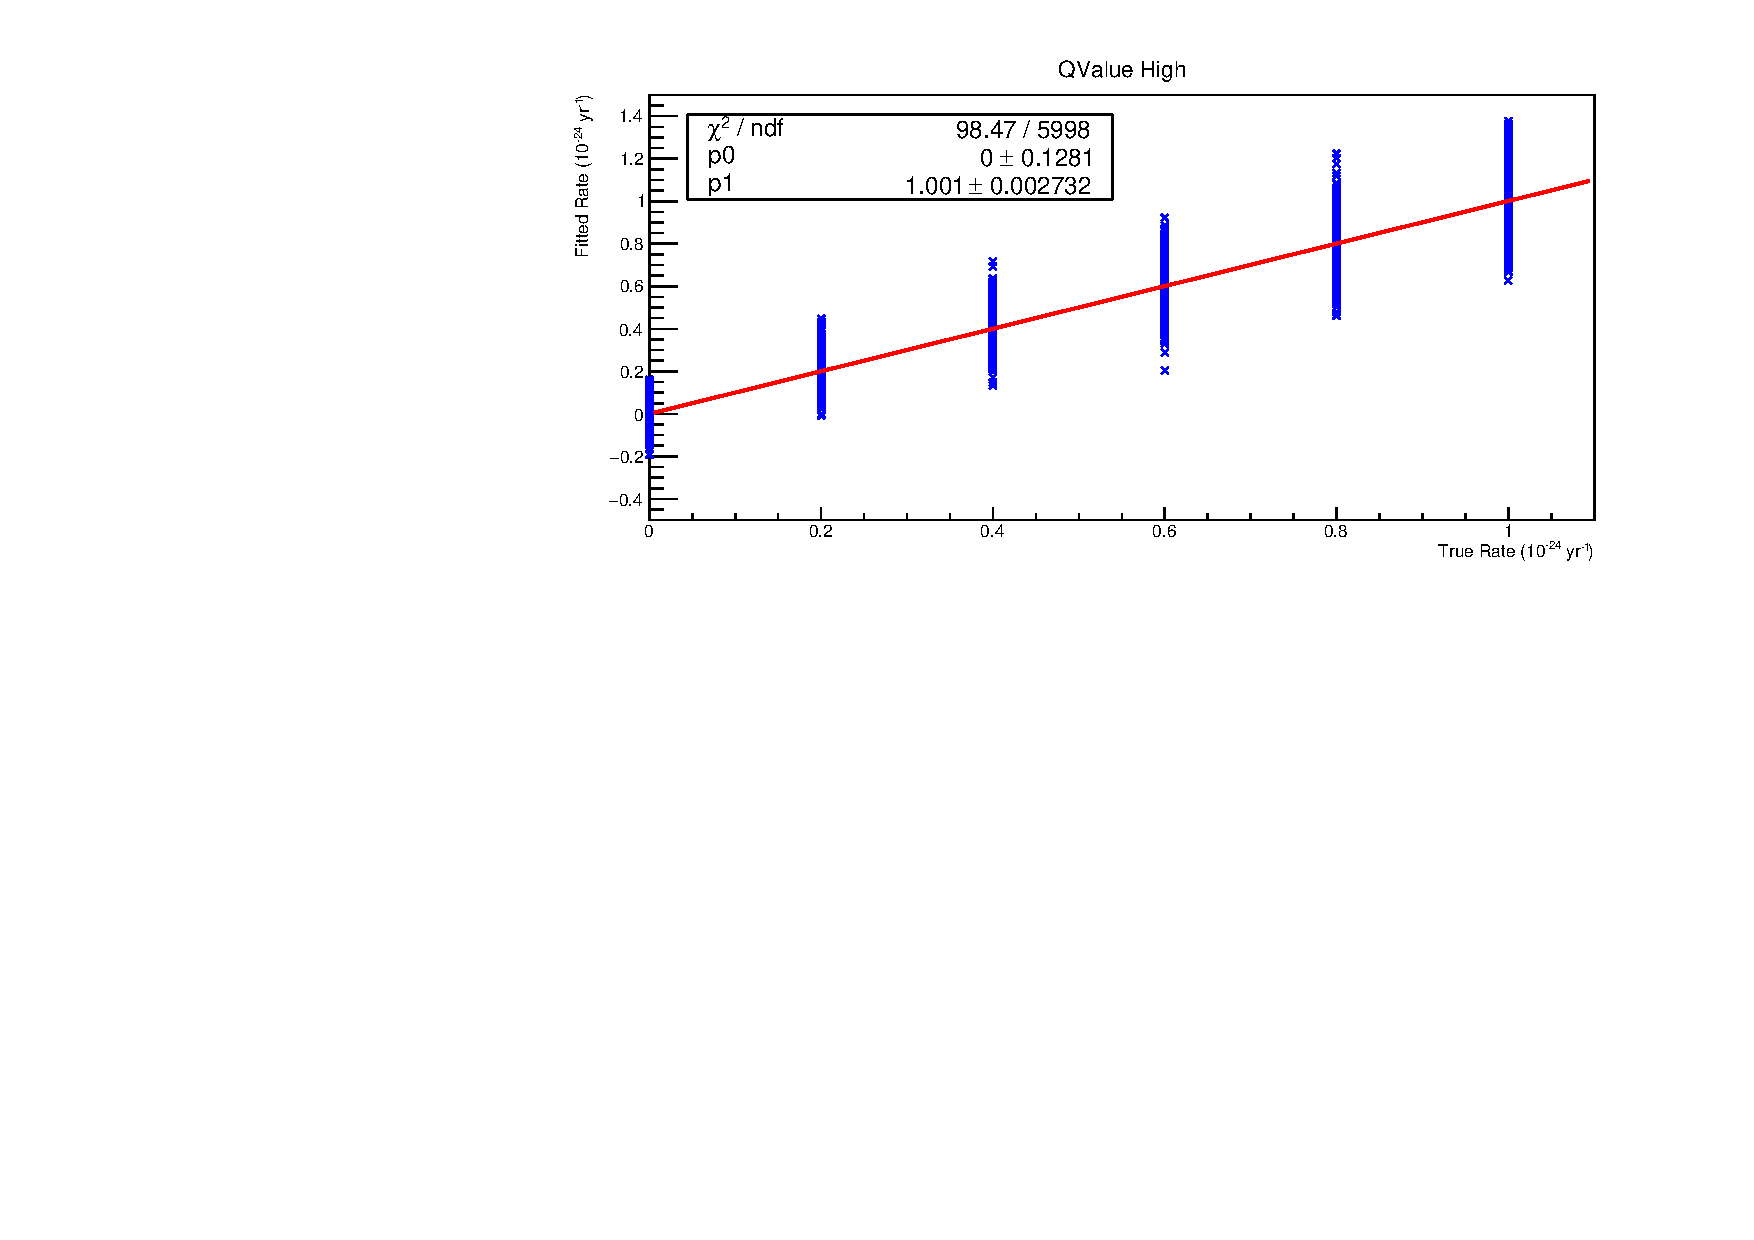
\includegraphics[width=0.7\linewidth]{Figures/Appendix_Figures/QValueHigh.pdf}
\caption[The fitted signal rate with the Q-value adjusted high]
{The fitted signal rate with the Q-value adjusted high.
The absolute bias is fixed to zero as it is the same case as in \autoref{fig:signalrate}, and a 0.2\% relative bias is applied from the error on the linear fit.}
\label{fig:qvaluehigh}
\end{figure}

\begin{figure}
\centering
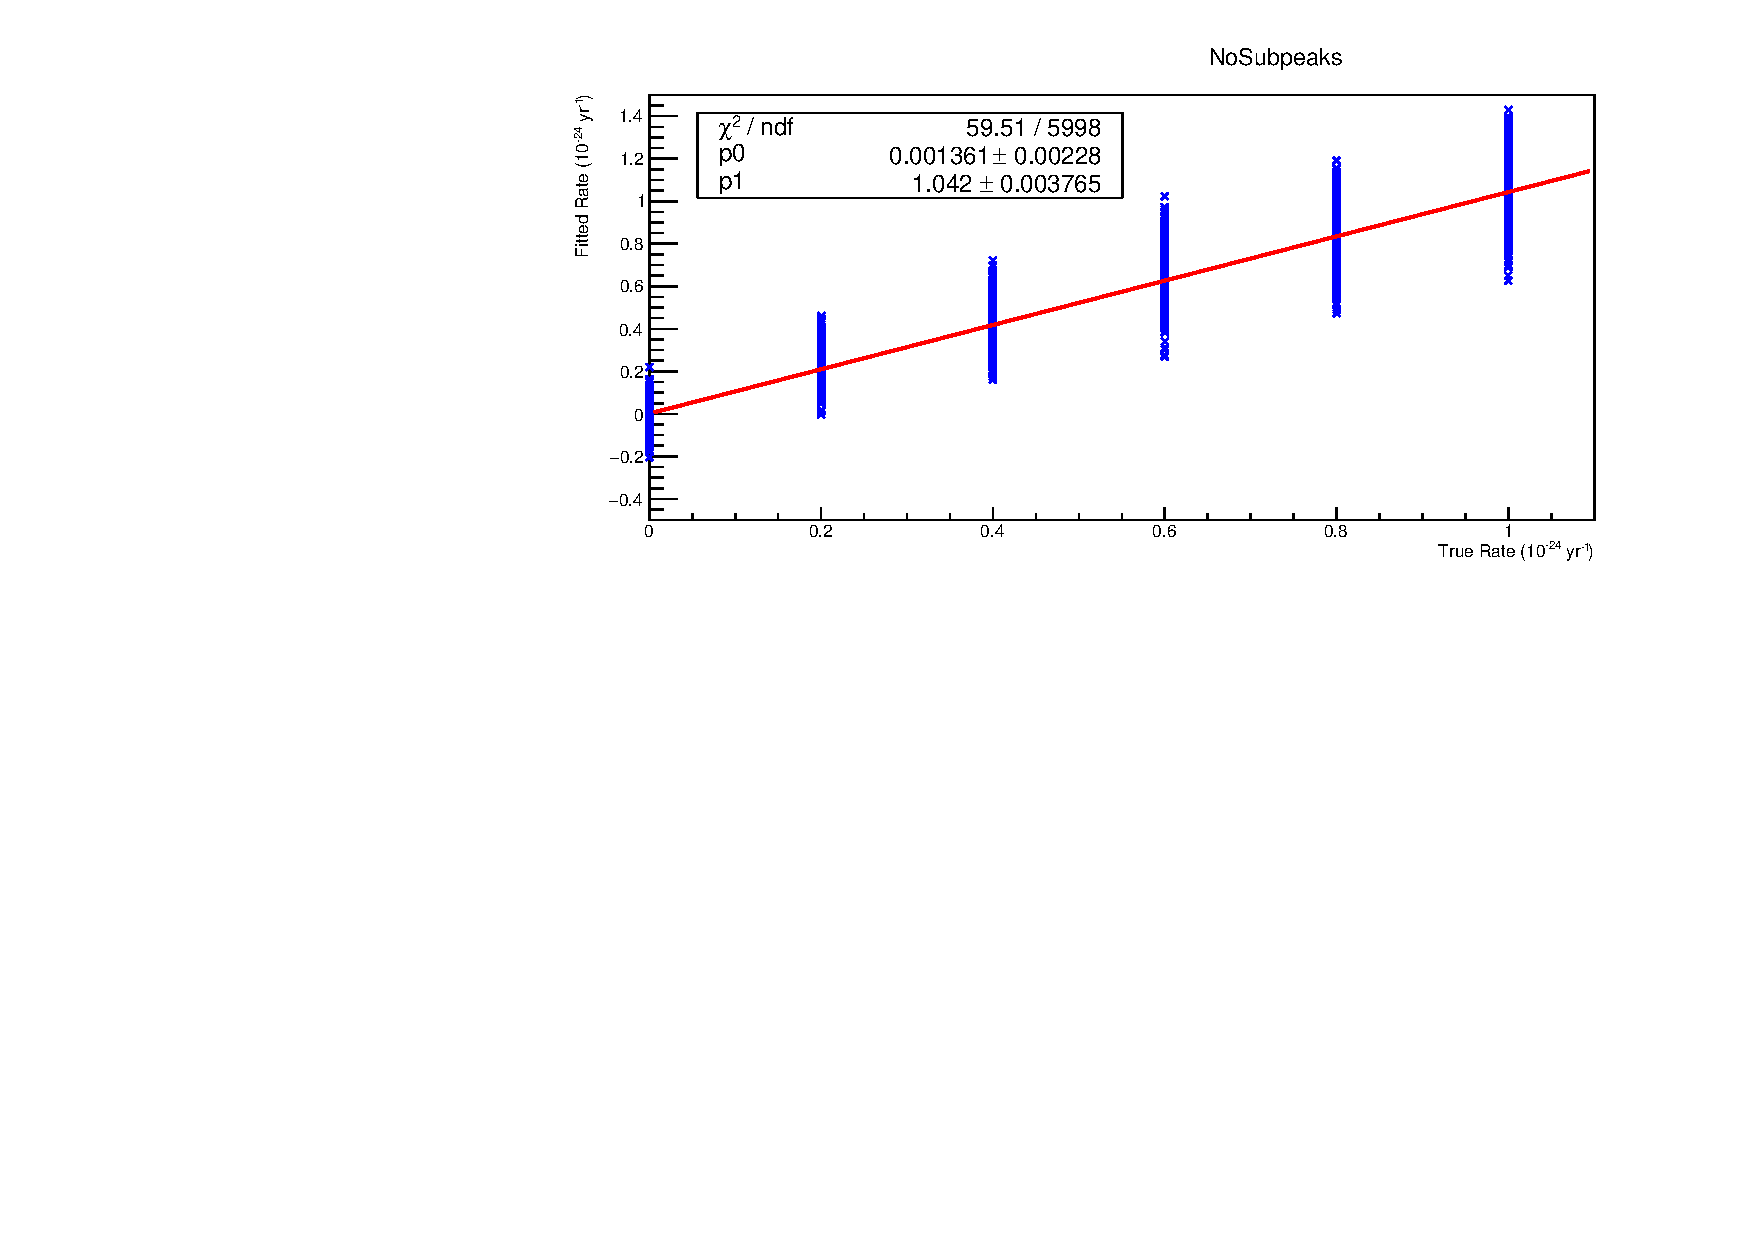
\includegraphics[width=0.7\linewidth]{Figures/Appendix_Figures/NoSubpeaks.pdf}
\caption[The fitted signal rate without taking into account subpeak parameters from the 2615 keV lineshape]
{The fitted signal rate without taking into account subpeak parameters from the 2615 keV lineshape.
For this parameter, both a relative and absolute bias is applied.
A flat prior is taken on the subpeak parameters, so the relative bias is taken to be 2.4\%.}
\label{fig:nosubpeaks}
\end{figure}